\documentclass[tikz,border=3pt]{standalone}
\usepackage{amsmath}
\usetikzlibrary{arrows.meta,fit,positioning,shapes.geometric}

\definecolor{textblue}{HTML}{2F5D8C}
\definecolor{visiongreen}{HTML}{2F7D6D}
\definecolor{gateorange}{HTML}{B66A1E}
\definecolor{routegray}{HTML}{66717E}
\definecolor{lossred}{HTML}{A6414A}

\tikzset{
  font=\sffamily\scriptsize,
  block/.style={
    draw,
    rounded corners=2pt,
    minimum height=9mm,
    align=center,
    inner sep=3pt,
    line width=.55pt
  },
  textblock/.style={block, draw=textblue, fill=textblue!8},
  visionblock/.style={block, draw=visiongreen, fill=visiongreen!8},
  gateblock/.style={block, draw=gateorange, fill=gateorange!10},
  headblock/.style={block, draw=routegray, fill=routegray!9},
  lossblock/.style={block, draw=lossred, fill=lossred!7},
  arrow/.style={-{Latex[length=2.2mm]}, line width=.65pt},
  dashedarrow/.style={arrow, dashed, draw=lossred},
  note/.style={align=center, text=routegray, font=\sffamily\tiny}
}

\begin{document}
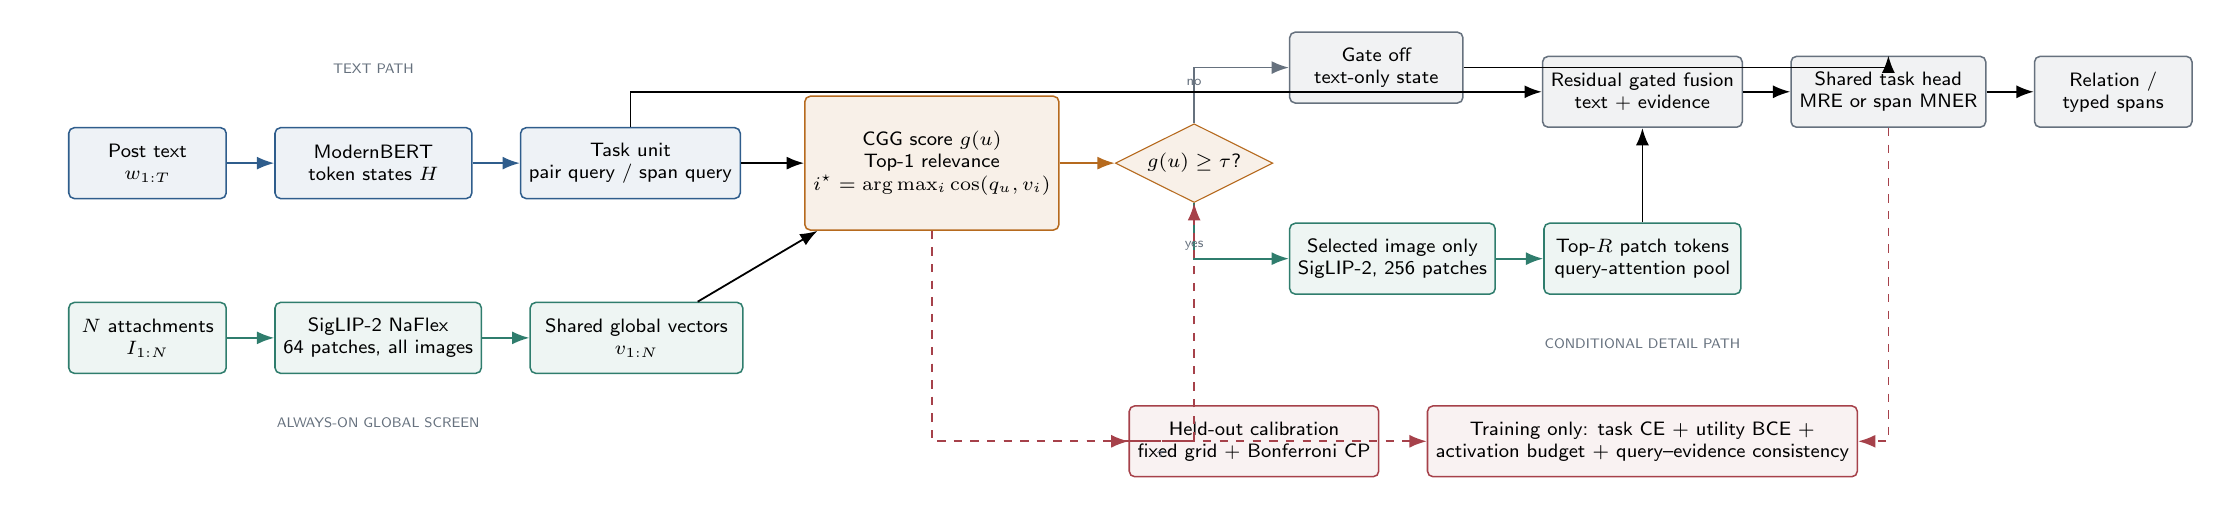
\begin{tikzpicture}[node distance=5mm and 6mm]
  \node[textblock, minimum width=20mm] (text) {Post text\\$w_{1:T}$};
  \node[textblock, right=of text, minimum width=25mm] (modernbert)
    {ModernBERT\\token states $H$};
  \node[textblock, right=of modernbert, minimum width=27mm] (unit)
    {Task unit\\pair query / span query};

  \node[visionblock, below=13mm of text, minimum width=20mm] (images)
    {$N$ attachments\\$I_{1:N}$};
  \node[visionblock, right=of images, minimum width=25mm] (screen)
    {SigLIP-2 NaFlex\\64 patches, all images};
  \node[visionblock, right=of screen, minimum width=27mm] (global)
    {Shared global vectors\\$v_{1:N}$};

  \node[gateblock, right=8mm of unit, minimum width=25mm, minimum height=17mm]
    (router) {CGG score $g(u)$\\Top-1 relevance\\$i^\star=\arg\max_i\cos(q_u,v_i)$};

  \node[diamond, draw=gateorange, fill=gateorange!10, aspect=2.0,
        right=7mm of router, align=center, inner sep=1.5pt] (decision)
    {$g(u)\geq\tau$?};

  \node[headblock, above right=5mm and 7mm of decision,
        minimum width=22mm] (off) {Gate off\\text-only state};
  \node[visionblock, below right=5mm and 7mm of decision,
        minimum width=25mm] (detail)
    {Selected image only\\SigLIP-2, 256 patches};
  \node[visionblock, right=of detail, minimum width=25mm] (regions)
    {Top-$R$ patch tokens\\query-attention pool};
  \node[headblock, above=12mm of regions, minimum width=25mm] (fusion)
    {Residual gated fusion\\text + evidence};
  \node[headblock, right=of fusion, minimum width=24mm] (taskhead)
    {Shared task head\\MRE or span MNER};
  \node[headblock, right=of taskhead, minimum width=20mm] (output)
    {Relation /\\typed spans};

  \draw[arrow, draw=textblue] (text) -- (modernbert);
  \draw[arrow, draw=textblue] (modernbert) -- (unit);
  \draw[arrow, draw=visiongreen] (images) -- (screen);
  \draw[arrow, draw=visiongreen] (screen) -- (global);
  \draw[arrow] (unit) -- (router);
  \draw[arrow] (global) -- (router);
  \draw[arrow, draw=gateorange] (router) -- (decision);
  \draw[arrow, draw=routegray] (decision) |- node[note, near start, above]{no} (off);
  \draw[arrow, draw=visiongreen] (decision) |- node[note, near start, below]{yes} (detail);
  \draw[arrow, draw=visiongreen] (detail) -- (regions);
  \draw[arrow] (regions) -- (fusion);
  \draw[arrow] (unit) |- (fusion);
  \draw[arrow] (off) -| (taskhead);
  \draw[arrow] (fusion) -- (taskhead);
  \draw[arrow] (taskhead) -- (output);

  \node[lossblock, below=14mm of regions, minimum width=53mm] (loss)
    {Training only: task CE $+$ utility BCE $+$\\activation budget $+$ query--evidence consistency};
  \node[lossblock, left=of loss, minimum width=30mm] (calibration)
    {Held-out calibration\\fixed grid + Bonferroni CP};
  \draw[dashedarrow] (taskhead) |- (loss);
  \draw[dashedarrow] (router) |- (loss);
  \draw[dashedarrow] (router) |- (calibration);
  \draw[dashedarrow] (calibration) -| node[note, below, near start]{$\tau$} (decision);

  \node[note, fit=(text)(modernbert)(unit), above=1mm of modernbert]
    {TEXT PATH};
  \node[note, fit=(images)(screen)(global), below=1mm of screen]
    {ALWAYS-ON GLOBAL SCREEN};
  \node[note, fit=(detail)(regions), below=1mm of regions]
    {CONDITIONAL DETAIL PATH};
\end{tikzpicture}
\end{document}
